\documentclass[dvipdfmx]{jsarticle}
\usepackage[T1]{fontenc}
\usepackage[dvipdfmx]{hyperref}
\usepackage{lmodern}
\usepackage{latexsym}
\usepackage{amsfonts}
\usepackage{amssymb}
\usepackage{mathtools}
\usepackage{nccmath}
\usepackage{amsthm}
\usepackage{multirow}
\usepackage[dvipdfmx]{graphicx}
\usepackage{wrapfig}
\usepackage{here}
\usepackage{float}
\usepackage{ascmac}
\usepackage{url}

\title{CGによるスタイル表現の比較と実験}
\author{文理学部情報科学科\\5419045 高林 秀}
\date{\today}

\begin{document}

\maketitle

\begin{abstract}
  本稿では、今年度マルチメディア情報処理の第2回目課題研究として、「blender」及び「Google Colabratory」における3DCGの描画をもちいて、配布されたデータ「Lit-Sphire」と[StyleBlit]を使用しCG画像のスタイル表現の動画化を実験し、それぞれのデータにおける結果を比較・考察するものである。結果は、、、、で、、、であった。
\end{abstract}

\section{目的}
本稿では、今年度マルチメディア情報処理の第2回課題研究としてCGスタイル表現を、レンダリング画像の連番データ化し、最終的には動画化をする実験を行う。本実験は、予め配布されたデータである、「Lit-Sphire」と[StyleBlit]を使用して行う。なお、実験環境はCGレンダリングソフト「brender」及び、クラウド上のPython環境である「GoogleColaboratory」を利用した。なお計算機スペックについては、後述する実験準備の章をご覧頂きたい。
\section{使用環境の紹介}
まずは、本実験で使用したソフトウェア、サービスについて軽く説明する。
\subsection{blenderについて}
blenderとは、オープンソースの統合型3DCGソフトウェアで、主に3Dモデリング、モーショングラフィックス、アニメーションやシミュレーション、レンダリングやデジタル合成など、3DCGにおける様々な機能を提供するソフトウェアである。WindowsからMacOS、Linux系のOSなど幅広く対応している。主な開発言語は、Python, C, C++。\par
開発元はBlenderFoundation(Blender財団)と呼ばれる非営利団体が行っており、この財団は短編コンピュータアニメーション映画の制作も行っている。\par
blenderは、一般的な3DCGソフトウェアの中では比較的軽量であり、ライセンス料も無料である。そのためプロ層に限らずアマチュア層や素人でも3DCGを体験することが可能だ。\par
blenderは、実際の映画制作スタジオでも広く利用されつつあり、近年の代表的な例だとスタジオカラー\footnote{日本のアニメーション制作会社である株式会社カラーの制作スタジオ。アニメーション制作会社ガイナックスの元取締役である庵野秀明氏が2006年5月に同社取締役を辞任し設立。社名である「カラー」はギリシャ語の「$\chi \alpha \rho \acute{\alpha}$(歓喜)」に由来。}の作品「シン・エヴァンゲリオン劇場版:||」の制作にも利用された。
\begin{table}[H]
  \begin{center}
    \caption{blenderの推奨動作要件}
    \begin{tabular}{|c|l|} \hline
      部品&スペック要件\\ \hline
      CPU & 4コア以上の64bitプロセッサ \\
      GPU & VRAMが4GB以上のグラフィックプロセッサ \\
      RAM & 16GB以上 \\
      ディスプレイ解像度 & 1920$\times$1080以上(Full HD)\\ \hline
    \end{tabular}
    \label{hyo01}
  \end{center}
\end{table}
\begin{itemize}
  \item blender公式ページ:\url{https://blender.org/}
\end{itemize}
\begin{figure}[H]
  \centering
  
\includegraphics[scale=0.4]{images/Logo_Blender.svg.png}
  \caption{blenderロゴ}
  出典:\url{https://ja.wikipedia.org/wiki/Blender_Foundation}
\end{figure}
\subsection{GoogleColaboratoryについて}
GoogleColaboratory(以降Colab)とは、自身のPC上にPythonの環境構築を行うことなくPythonを利用することができるGoogleのサービスである。Microsoft Edgeや、Google Chromeなどのウェブブラウザで動作するため、初心者から上級者まで幅広くPythonを利用した開発を行うことができる。Colabは、機械学習の普及を目的としたサービスである。\par 見た目は、JupyetrNoteBook\footnote{ブラウザ上で動作する、対話型のPython実行環境。Anacondaに付属している。}のウェブブラウザ版だと思って良い。Googleアカウントさえあれば誰でも無料で使用でき、機械学習等でCPU以外のプロセッサを利用したい場合はGPU\footnote{GPU:Graphics Processing Unitの略。画像処理に特化したプロセッサ。コンピュータが画面に描画する映像の計算処理を主な任務としている。そのため、CPUよりも単純構造でコアを大量に積んでいるため、並列計算に特化している。代表的なGPUには、Nvidea社のGEFORCEがある。}やTPU\footnote{TPU:Tensor processing Unitの略
。Googleが開発した、機械学習に特化した集積回路(ASIC)。GPUより1ワットあたりのIOPSが高いが、計算精度は劣る。}も無料で利用することが可能だ。\par
Colabはブラウザがあれば動作するため、スマートフォンやタブレット端末からでも利用することができる。したがって機種に依存せず、複数人と共有して利用することが可能となる。
\begin{figure}[H]
  \centering
  
\includegraphics[scale=0.4]{images/colab_logo.jpeg}
  \caption{Colabロゴ}
  出典:\url{https://www.tcom242242.net/entry/%E3%83%A1%E3%83%A2/colab/%E3%80%90%E5%85%A5%E9%96%80%E3%80%91colaboratory%E3%81%AE%E5%A7%8B%E3%82%81%E6%96%B9/}
\end{figure}
\begin{itemize}
  \item Colabホームページ:\url{https://colab.research.google.com/notebooks/welcome.ipynb?hl=ja}
\end{itemize}
\section{関連技術調査}
今回配布されてたデータ「Lit-Sphire」と[StyleBlit]について説明する。\par
なお事前に説明すると、テクスチャとは、「3Dオブジェクトンの凹凸や色の画像」のことで、マッピングとは「テクスチャを3Dオブジェクトに貼り付けること」をそれぞれ意味する。
\subsection{Lit-Sphire}
Lit-Sphireとは、3Dシェーディング\footnote{}の手法において、球状の環境マップ\footnote{3DCGにおけるテクスチャマッピングの手法の1つ。3D上の表面に擬似的な周囲環境の映り込みを再現する手法。}利用したシェーディングの手法のことである。この手法では、材質と光を表現した球状の絵を利用し、擬似的にライティングを行っている。したがって、事前にライティングの計算を済ませてから、適用先オブジェクトへのライティングを行っている。
\begin{figure}[H]
  \centering
  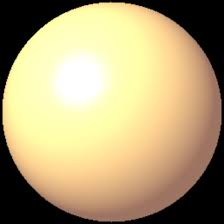
\includegraphics[scale=0.4]{images/lit_demo.png}
  \caption{球状環境マップの一例}
  出典:\url{https://mevislabdownloads.mevis.de/docs/current/MeVisLab/Standard/Documentation/Publish/ModuleReference/SoGVRLitSphereShading.html}
\end{figure}
Lit-Sphreは、ユーザーからそのオブジェクトが見える位置であるカメラ座標の法線座標をテクスチャの座標として使用し、法線と環境マップの色の対応付けを行う役割を果たす。テクスチャ画像の RGB 値が「面の向き」を示している。R 値が右側の面の向きを示し、G値が上側の面の向きを示している。この面の向きと、マテリアル画像の位置関係の対応を計算し、その色を構成画像上に張り付けることで、レンダリングしている。\par
 
本稿では取り扱わないが、他のシェーディング手法であるLambertシェーディングや、Phongシェーディングとは違い環境マップを使用して直感的に色を成業する事ができるので、NPR\footnote{NPR:Non Photorealistic renderingの略。和訳は「非写実的レンダリング」。}目的として都合が良いシェーダーであるとされる。\par
ところで、NPRとは反対の目的で「PR:Photorealistic rendering」と呼ばれるものがあるが、これは「物理現象のシュミレーションにより、より現実見のある(写実的な)CGレンダリング」を目的として行われる。
\begin{figure}[H]
  \centering
  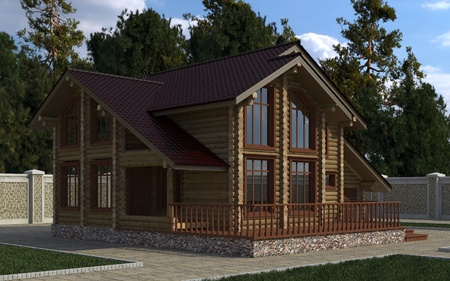
\includegraphics[scale=0.4]{images/PR.jpg}
  \caption{PRの一例}
  出典:\url{https://jp.123rf.com/photo_85627230_%E5%AE%B6%E3%81%AE%E5%86%99%E5%AE%9F%E7%9A%84%E3%81%AA%E3%83%AC%E3%83%B3%E3%83%80%E3%83%AA%E3%83%B3%E3%82%B0%E3%81%AE-3-d-%E5%9B%B3.html}
\end{figure}
上図のように精密な写実的なCGモデルを構築するには、被写体のモデルも精密である必要がある。対して、NPRは絵画や、イラスト等のあまり現実味のない(非写実的)な画像、CGを構築することを示す。人が描く絵を書くようにCGを構築することを指す。
\begin{figure}[H]
  \centering
  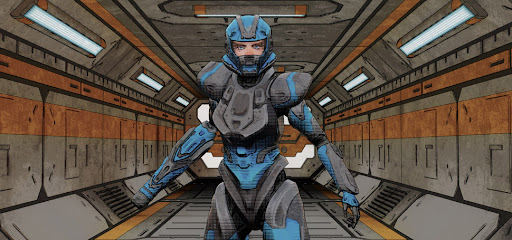
\includegraphics[scale=0.4]{images/NPR.jpg}
  \caption{NPRの一例}
  出典:\url{http://modogroup.jp/modo/kits/npr}
\end{figure}
\subsection{StyleBlit}
レンダリングには、通常比較的強いマシンスペックが要求されることが多い。しかし、Sty5leBlitと呼ばれるレンダリング手法は、1コアのCPUでも高品質なレンダリングを提供することのできる技術、アルゴリズムとなっている。\par
StyleBlitとは、高品質で定型化されたレンダリングを提供できる効率的なスタイル転送アルゴリズムである。このStyleBlitは比較的計算量の少ないゲームやモバイル系のアプリに適したアルゴリズムとなっている。\par
StyleBlitに関して、藤堂英樹氏のブログ\cite{bib01}にて非常に分かりやすく紹介されているので、引用する。
\begin{quote}
  StyleBlitは,Lit-Sphereと同様に,球にデザインされたシェーディングを3Dモデル上に転写できますが,ストロークのような細かい特徴まで合わせて転写することが可能です.
\end{quote}
つまり、StyleBlitはLit-Sphereと同様に球状の環境マップを利用したシェーディングの手法と言うことになる。では、実際のレンダリングにおいて、両者にはどの様な相違点があるのか。同氏のブログ\cite{bib01}には次のように述べられている。
\begin{quote}
  通常のLit-Sphereだと,下記のようなストロークタッチ込みのマップは法線マップの影響で歪んでしまってうまく転写できませんが,StyleBlitだと歪みなく転写することができます.
  \begin{figure}[H]
    \centering
    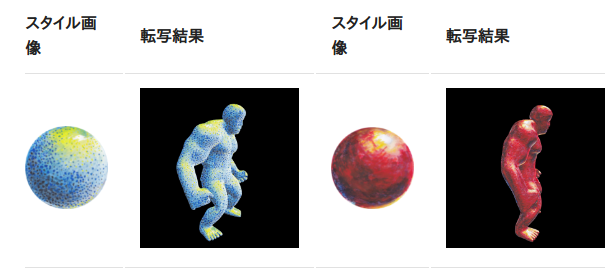
\includegraphics[scale=0.4]{images/todoteacher.png}
  \end{figure}
\end{quote}
つまり、Lit-Sphireでは歪んでしまうような部分でも、StyleBlitを利用することで鮮明に歪みなくレンダリングをすつことができるという点で、両者は大きく異なっていると言える。\par
巻末付録に、StyleBlitの開発者ホームページへのリンクを載せる。必要に応じてご参照いただきたい。
\paragraph{手法解説}
以下、同氏のブログに記載されている内容を踏襲しながらStyleBlitの流れを説明する。その前に、3Dレンダリングで何かと登場することの多い「法線マップ」とはなにか説明する。\par
法線マップとは、ポリゴン\footnote{ポリゴン:曲面を構成する最小単位。英語では「Polygon」。多角形という意味。3DCGにおいて、3点以上の頂点を結んで得られる多角形データのこと。}に対して、貼り付けることのできるテクスチャの画像データとは別に専用の画像データで割り当てることのできる、法線ベクトルの集合データのことである。法線はポリゴン上の凹凸の影を表現するのに利用され、3Dオブジェクトの1枚のテクスチャ上に対する、光の入射方向と法線マップ上の法線の方向、すなわち法線ベクトルを元に計算している。\par
\begin{figure}[H]
  \centering
  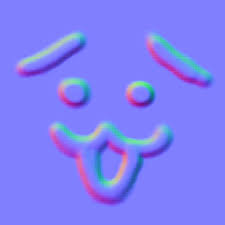
\includegraphics[scale=0.4]{images/hosenmap.jpeg}
  \caption{法線マップの一例}
  出典:\url{https://nodachisoft.com/common/jp/article/jp000050/}
\end{figure}
StyleBlitでは、スタイル転写を実行する時ガイド画像とよばれる法線画像を用いて特徴の類似する部分を探索する。このとき、法線のガイド画像等を入力し、RGBの画像を出力する。
以下アルゴルズムの概要を示す。\par
\begin{itemize}
  \item 入力一覧
  \begin{itemize}
    \item $C_{S}$:スタイル画像(RGB)
    \item $G_{S}$:スタイルガイド画像(法線画像)
    \item $G_{T}$:ターゲットガイド画像(法線画像)
  \end{itemize}
  \item 出力
  \begin{itemize}
    \item $C_{T}$:ターゲット画像
  \end{itemize}
\end{itemize}
出力画像$C_{T}$のピクセル$p$の色値(RGB)$C_{T}(p)$は次に示す手順で算出される。
\begin{enumerate}
  \item ターゲットガイド画像の法線空間におけるピクセルの色$G_{T}(p)$の特徴に類似するパッチ領域$p \in \Omega_{T_{i}}$を考える。
  \item 上記バッチ領域における代表点$q$を計算する。
  \item 代表点$$q$のターゲットガイド画像の法線$G_{T}(q)$に類似する法線を持つピクセル$u$をスタイルガイド画像$G_{S}$の法線$G_{S}(u)$から探索する。
  \item $u$を中心としたパッチ領域$u \in \Omega_{S_{i}}$を考える。
  \item スタイル画像のピクセルのRGB値を$C_{S}(u)$とし、ターゲット画像側に$C_{S}(u)$を以下の形で転写する。
  \begin{gather*}
    C_{T}(p) = C_{S}(u + p -q)
  \end{gather*}
\end{enumerate}
以下の画像は、開発者がYoutube上に公開しているStyleBlitの概要動画における、MatCapとの比較シーンにおける一部場面である。
\begin{figure}[H]
  \centering
  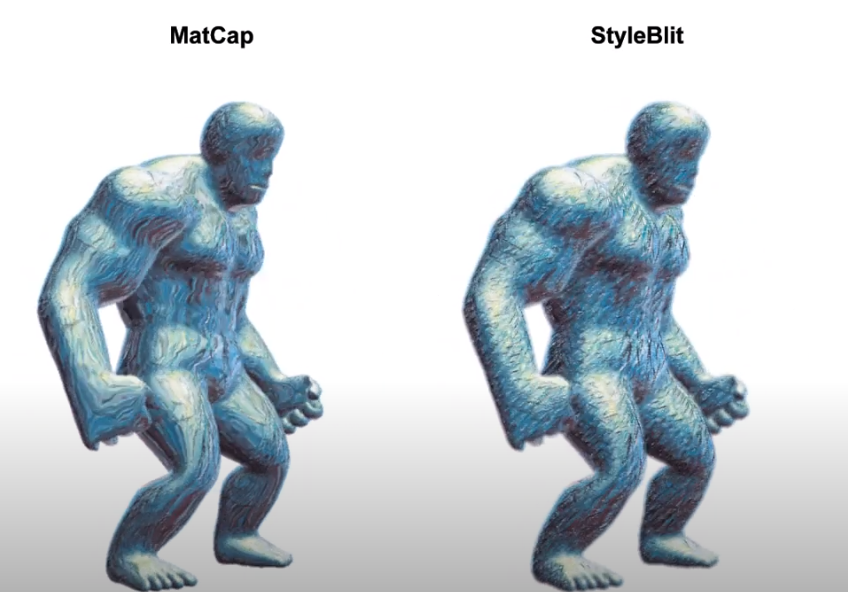
\includegraphics[scale=0.4]{images/styleblit_ex.png}
  \caption{MatCapとStyleBlitの比較}
  出典:\url{https://www.youtube.com/watch?v=krQrDhestVA&t=1s}
\end{figure}
上記を見ると確かに、オブジェクトの表面の歪みがStyleBlitの方が無いことが伺える。
\section{実験方法}
まず、本実験の目標を改めて説明する。本実験は「Lit-SphereとStyleBlitのスタイル表現をレンダリング画像の連番データに適用する」ことを目的とする。
  \subsection{実験準備}
  \paragraph{実験環境}
    今回の実験は以下の環境上で行った。下記に実験時の環境を示す。
    \begin{itemize}
      \item OS:Window10 Home Ver.20H2
      \item CPU:Intel(R)Core(TM)i7-9700K 8cores @ 3.6GHz
      \item GPU:Nvidia Geforce RTX2070 OC VRAM 8GB
      \item RAM:16GB
      \item brenderのバージョン:2.93.1
      \item Chromeのバージョン: 92.0.4515.107
    \end{itemize}
  \subsection{実験手順}
  まず、スタイル表現を動画化する全体的な流れは以下の通りである。
  \begin{enumerate}
    \item blenderファイルより連番画像を制作
    \item 配布されたColabノートブックにて上記画像を1枚ずつスタイル化処理
    \item スタイル化した画像を動画化
  \end{enumerate}
  以下具体的な流れを説明する。
  \begin{enumerate}
    \item 配布されたスライド資料にしたがって、blenderで連番画像を出力し、結果をZIP形式で圧縮し一つにまとめておく。
    \item 以下、配布されたColabノートブックにある「必要なライブラリのインストール」のコードセルを実行する。
    \item ライブラリのインストールが完了したら、画像ベースのスタイル化の実装例と補助関数のコードセルをそれぞれ順番に実行する。
    \item 必要なファイルをColab上にアップロードする。
    \begin{itemize}
      \item 左のサイドバーからフォルダのアイコンをクリックし、「セッションストレージにアップロード」を選択し、エクスプローラーからファイルを選択する。
    \end{itemize}
    \item ファイルのアップロードが完了したらColabの入力画像の設定にある指示にしたがって、必要なパラメータを指定し、コードセルを実行する。
    \item ColabのLit-Sphere/StyleBlitの結果の確認からそれぞれのレンダリング手法による結果を確認し、考察を行う。
    \item ColabのLit-Sphere/StyleBlitの動画出力結果のコードセルをそれぞれ実行し、動画化を行う。その結果を確認し、考察を行う。
  \end{enumerate}
\section{実験結果}
以下、スタイル化結果のスクリーンショットを示す。
\subsection{モデル:suzanneの場合}
テクスチャ画像が左で、転写するモデルが右側に示されている。
\begin{figure}[H]
  \centering
  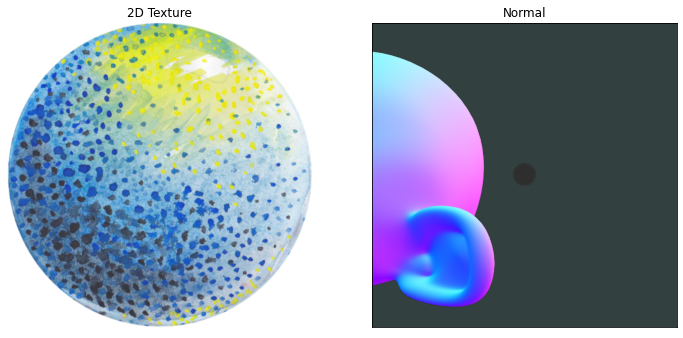
\includegraphics[scale=0.4]{images/suzzanne_input1.png}
  \caption{入力画像1}
\end{figure}
\begin{figure}[H]
 \begin{minipage}{0.5\hsize}
  \begin{center}
   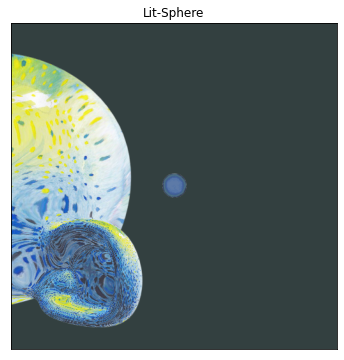
\includegraphics[scale=0.4]{images/suzzanne_lit_out1.png}
  \end{center}
  \caption{Lit-Sphireでの出力結果画像}
 \end{minipage}
 \begin{minipage}{0.5\hsize}
  \begin{center}
   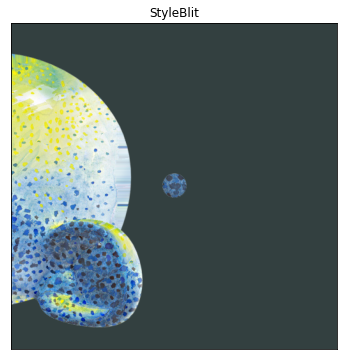
\includegraphics[scale=0.4]{images/suzzanne_style_out1.png}
  \end{center}
  \caption{StyleBlitでの出力結果画像}
 \end{minipage}
\end{figure}
なおこの条件での動画出力結果は、以下のリンクから参照できる。
\begin{itemize}
  \item URL:\url{https://drive.google.com/drive/folders/112dBLmxLyQe94MToRBUOHlm75C4zrxKg?usp=sharing}
\end{itemize}

次に、テクスチャを変更して同様の実験を行った。その時の結果は下記。
\begin{figure}[H]
  \centering
  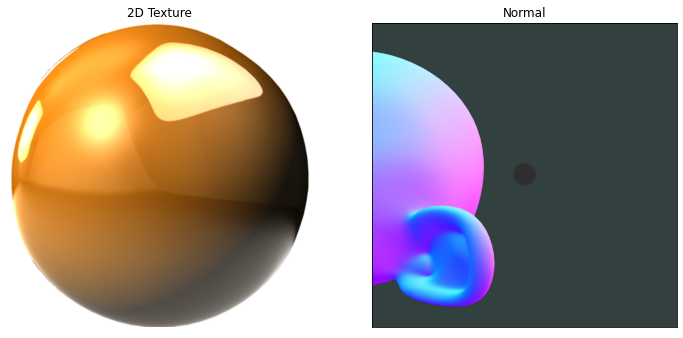
\includegraphics[scale=0.4]{images/suzzanne_input2.png}
  \caption{入力画像2}
\end{figure}
\begin{figure}[H]
 \begin{minipage}{0.5\hsize}
  \begin{center}
   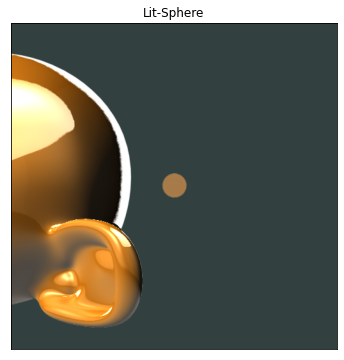
\includegraphics[scale=0.4]{images/suzzanne_lit_out2.png}
  \end{center}
  \caption{Lit-Sphireでの出力結果画像}
 \end{minipage}
 \begin{minipage}{0.5\hsize}
  \begin{center}
   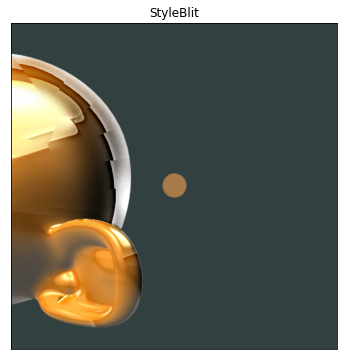
\includegraphics[scale=0.4]{images/suzzanne_sytle_out2.png}
  \end{center}
  \caption{StyleBlitでの出力結果画像}
 \end{minipage}
\end{figure}
なおこの条件での動画出力結果は、以下のリンクから参照できる。
\begin{itemize}
  \item URL:\url{https://drive.google.com/drive/folders/1L7WVmp5V8TFQB9ILghPZwqvu1XI9gEQv?usp=sharing}
\end{itemize}
\subsection{モデル:blobbyの場合}
また、異なる3Dモデルでも同様の実験を行ってみた。
\begin{figure}[H]
  \centering
  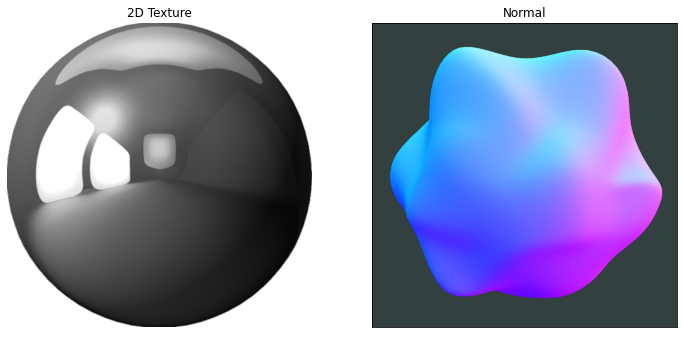
\includegraphics[scale=0.4]{images/blo_input1.png}
  \caption{入力画像3}
\end{figure}
\begin{figure}[H]
 \begin{minipage}{0.5\hsize}
  \begin{center}
   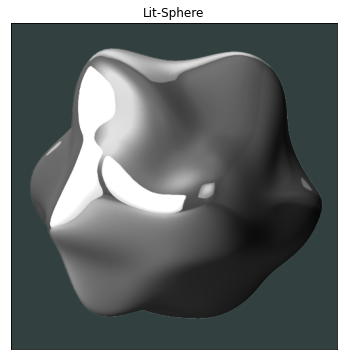
\includegraphics[scale=0.4]{images/blo_lit_out3.png}
  \end{center}
  \caption{Lit-Sphireでの出力結果画像}
 \end{minipage}
 \begin{minipage}{0.5\hsize}
  \begin{center}
   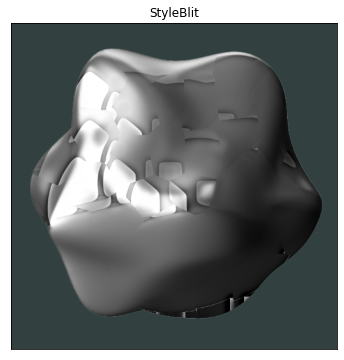
\includegraphics[scale=0.4]{images/blo_stylr_out3.png}
  \end{center}
  \caption{StyleBlitでの出力結果画像}
 \end{minipage}
\end{figure}
なおこの条件での動画出力結果は、以下のリンクから参照できる。
\begin{itemize}
  \item URL:\url{https://drive.google.com/drive/folders/1fics3oMdK64yPkb5z2NB42zhTQyoBngQ?usp=sharing}
\end{itemize}
加えて、異なるテクスチャでも同様の実験を行ってみた。
\begin{figure}[H]
  \centering
  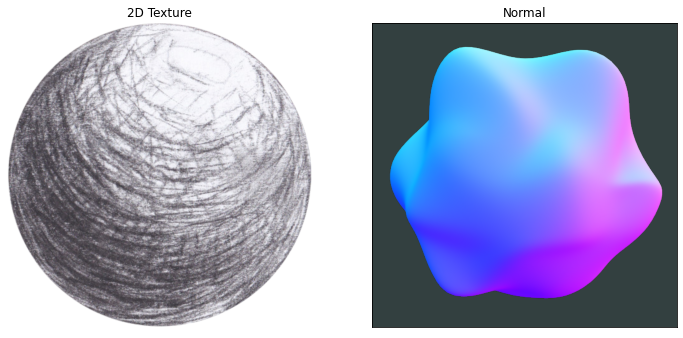
\includegraphics[scale=0.4]{images/blo_input4.png}
  \caption{入力画像4}
\end{figure}
\begin{figure}[H]
 \begin{minipage}{0.5\hsize}
  \begin{center}
   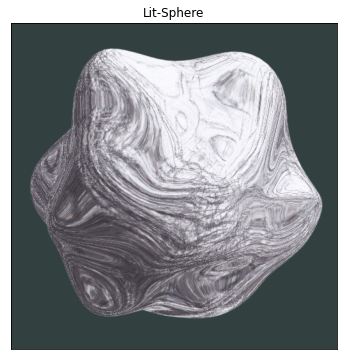
\includegraphics[scale=0.4]{images/blo_lit_out4.png}
  \end{center}
  \caption{Lit-Sphireでの出力結果画像}
 \end{minipage}
 \begin{minipage}{0.5\hsize}
  \begin{center}
   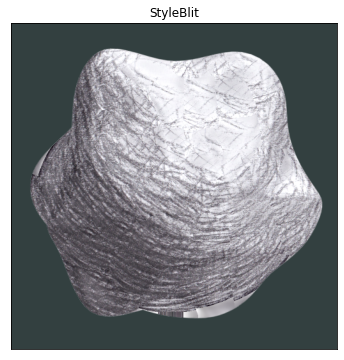
\includegraphics[scale=0.4]{images/blo_style_out4.png}
  \end{center}
  \caption{StyleBlitでの出力結果画像}
 \end{minipage}
\end{figure}
なおこの条件での動画出力結果は、以下のリンクから参照できる。
\begin{itemize}
  \item URL:\url{https://drive.google.com/drive/folders/1wMASt-w3BbsDIBcSFDGM8_pVyUbzJpUO?usp=sharing}
\end{itemize}


\section{考察}
\section{まとめ}


\section{巻末付録}
\begin{itemize}
  \item StyleBlit開発者ページリンク:\url{https://dcgi.fel.cvut.cz/home/sykorad/styleblit.html}
  \item GoogleDriveへのリンク:\url{https://drive.google.com/drive/folders/1ciY7XHNFSsUBXfiAC9xqw2D2_LYDKVSv?usp=sharing}
  \item GitHubリポジトリはこちら:\url{https://github.com/tsyu12345/Multi-report2}
\end{itemize}
\begin{thebibliography}{99}
  \bibitem{bib01} 藤堂英樹、『研究開発日誌』よりStyleBlit、(2019.7.30)、\url{http://hideki-todo.com/cgu/blog/article/styleblit/}
\end{thebibliography}

\end{document}
